\section{Auswertung}
\label{sec:Auswertung}
Die Graphen wurden sowohl mit Matplotlib als auch Numpy erstellt. Die
 Fehlerrechnung wurde mithilfe von Uncertainties durchgeführt.
 \begin{figure}
 	\centering
 	\caption{Die Temperaturverläufe des Wassers in den den Wärmereservoirs 1 und 2.}
 	\includegraphics[width=\linewidth-70pt,height=\textheight-70pt,keepaspectratio]{build/Temperaturen.pdf}
 	\label{fig:Graph1}
 \end{figure}
 \begin{figure}
 	\centering
 	\caption{Der Temperaturverlauf im ersten Reservoir und seine Approximation durch ein Polynom 2. Grades in Abhängigkeit der Zeit.}
 	\includegraphics[width=\linewidth-70pt,height=\textheight-70pt,keepaspectratio]{build/T1.pdf}
 	\label{fig:Graph1}
 \end{figure}
 \begin{figure}
 	\centering
 	\caption{Der Temperaturverlauf im zweiten Reservoir und seine Approximation durch ein Polynom 2. Grades in Abhängigkeit der Zeit.}
 	\includegraphics[width=\linewidth-70pt,height=\textheight-70pt,keepaspectratio]{build/T2.pdf}
 	\label{fig:Graph1}
 \end{figure}
 \begin{figure}
 	\centering
 	\caption{Der Verlauf der Dampfdruckkurve des Transportgases Dichluorfluormethan in Abhängigkeit der reziproken Temperatur.}
 	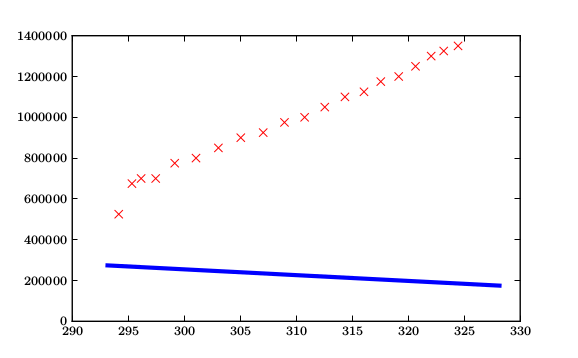
\includegraphics[width=\linewidth-70pt,height=\textheight-70pt,keepaspectratio]{build/Dampdruck.pdf}
 	\label{fig:Graph1}
 \end{figure}




 Zur Approximation des Temperaturverlaufes beim 1. Resservour wurde ein
 quadratischer Fit der Form $y = Ax+Bx+C$ verwendet. Eine nichtlineare
 Ausgleichsrechnung der Form $y = Ax+B+C$ liefert mit den im Minutentakt
 aufgenommenenen Temparaturdaten von Resservour 1 aus Tabelle \ref{tab:daten}
 die Parameter:$A = $,$B = $,$C =$

 \begin{table}
   \centering
   \input{build/tabges.tex}\label{tab:daten}
 \end{table}

 \begin{table}
   \centering
   \input{build/tabv.tex}\label{tab:daten}
 \end{table}
$A = 7.17334$

Durch Differentation folgen die Differenzenquotienten $\frac{\text{d}T_1}{\text{d}t}$ und $\frac{\text{d}T_2}{\text{d}t}$ der Form $y = Ax+B$ in Tabelle \ref{tab:dT}.

%Tabelle
Mithilfe von Formel \ref{eq:T1Q1} und \ref{eq:v} folgt die reale Güte an den in Tabelle \ref{tab:datv}:

\begin{table}
  \centering
  \input{build/tabv.tex}\label{tab:datv}
\end{table}
Mithilfe einer linearen Ausgleichsrechnung der Form $y=Ax+b$ mittels scipy folgt
$L$ aus den Daten von $\frac{1}{T2}$ und $\ln(Pb)$ mithilfe von Formel \ref{eq:L}
 \begin{equation}
   L = R*\frac{\text{d}y}{\text{d}x}\label{eq:L}
 \end{equation}
\begin{table}
  \centering
  \input{build/tabm.tex}\label{tab:datm}
\end{table}

\begin{table}
  \centering
  \input{build/tabn.tex}\label{tab:datn}
\end{table}
%nochne Tablle
